\documentclass{beamer}
%\usetheme{Madrid}
%\usetheme{Boadilla}
%\usetheme{default}
%\usetheme{Warsaw}
%\usetheme{Bergen}
%\usetheme{Frankfurt}
\usetheme{Darmstadt}

%\usecolortheme{seahorse}
%\usecolortheme{beaver}
\usecolortheme[named=orange]{structure}

\setbeamertemplate{footline}[page number]
%\setbeamercovered{transparent}
\setbeamercovered{invisible}
\setbeamertemplate{navigation symbols}{}

\usepackage{multimedia}
\usepackage{graphicx}
\usepackage[utf8]{inputenc}
%\usepackage[T1]{fontenc}
\usepackage[frenchb]{babel} 
\usepackage[all]{xy}
\usepackage{multirow}
\usepackage{lmodern}
\usepackage{subfigure}
\usepackage{ulem}
\usepackage{hyperref}

%% --------------

\title[Pr\'esentation Linux]{D\'ecouverte de Linux}
\author{L\'eo B\textsc{audouin}}
\institute[IFMA]
{
Pr\'esentation de Linux / Ubuntu\\
\medskip
{\emph{leo.baudouin@ifma.fr}}
}
\date{23 janvier 2012}

%% --------------

\begin{document}

\begin{frame}
\titlepage
\end{frame}

\begin{frame}
\tableofcontents
\end{frame}

%% --------------

\section{Historique}
\subsection{Dates importantes}
\begin{frame}
  \begin{block}{Chronologie :}
   ~~~~\begin{minipage}{\linewidth}
      \begin{itemize}
      \item[1969 :] Début du projet U\textsc{nix}
      \item[1984 :] Naissance du projet GNU
      \item[1985 :] Première branche du projet Windows
      \item[1991 :] Debut du projet \textit{Freax} par Linus Torvalds
      \item[1992 :] L'h\'ebergeur renomme le projet en Linux : Linus + UNIX
      \item[1994 :] Premier noyau stable pour le grand public
      \item[.\,\dots :] Optimisation du code de Linux
      \item[2010 :] Sortie de la version 10.04 LTS d'Ubuntu
      \item[2011 :] Sortie de la derniere version d'Ubuntu
      \end{itemize}
    \end{minipage}
  \end{block}
\end{frame}

\subsection{D\'eveloppement}
\begin{frame}
  \begin{block}{ Principales versions de Linux}

    ~~~~~~~~~~~~~~~~%
    \begin{minipage}[t]{0.85\linewidth}
      \begin{itemize}
      \item[Fedora :] Distribution communautaire supervisée par l'entreprise Red Hat
      \item[Mandriva :] La plus grande distribution européenne supervis\'e par l'entreprise du m\^eme nom
      \item[openSUSE :] Distribution principalement pour les entreprises supervis\'ee par Novell
      \item[Ubuntu :] Distribution grand public, communaut\'e tr\`es dynamique
      \end{itemize}
    \end{minipage}

  \end{block}

\vspace{5mm}
%\begin{center}
4 distributions mères :\\
\begin{enumerate}
\item Debian
\item Slackware
\item SuSE Linux
\item Red Hat Enterprise Linux
\end{enumerate}
%Chaque distribution a des d\'eriv\'ees afin de pouvoir \^etre d\'edi\'ees \`a des environnements particuliers tel que \textit{Edubuntu} pour l'\'education.
%\end{center}
\end{frame}

\subsection*{Noyau}
\begin{frame}
\begin{center}
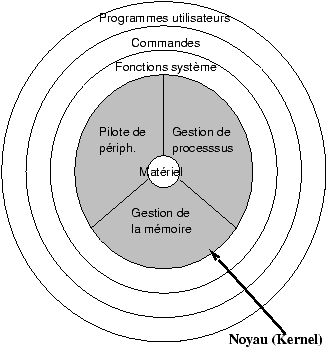
\includegraphics[width=0.4\linewidth]{images/kernel}
\begin{block}{Noyau commun}
Interface Matériel-Logiciel\\
Fonctions de base\\
Interface = Programme
\end{block}
\end{center}

\end{frame}

\subsection{\'Evolution graphique}
\begin{frame}
  \center Depuis la console jusqu'au tactile :
  \begin{figure}
    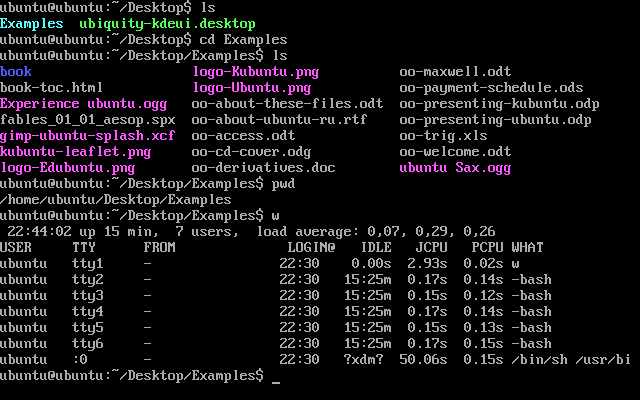
\includegraphics[width=0.8\linewidth]{images/console0}
    \caption{Console}
  \end{figure}
\end{frame}

\begin{frame}
  \center Premi\`eres interfaces graphiques
  \begin{figure}
    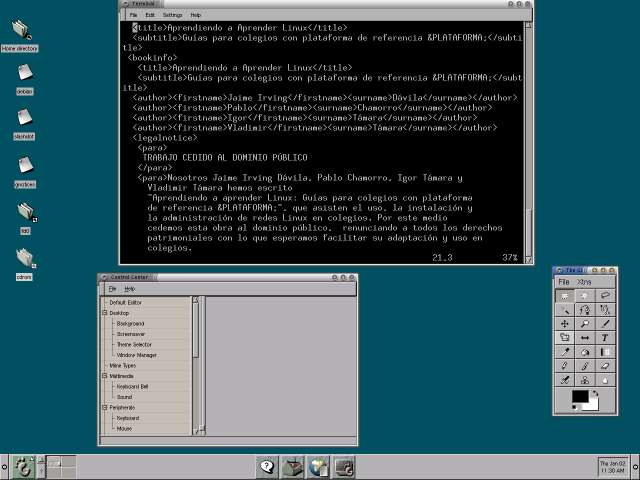
\includegraphics[width=0.8\linewidth]{images/GNOME-1999}
    \caption{Gnome en 1999}
  \end{figure}
\end{frame}

\begin{frame}
  \center Interface con\c{c}ue pour le tactile
  \begin{figure}
    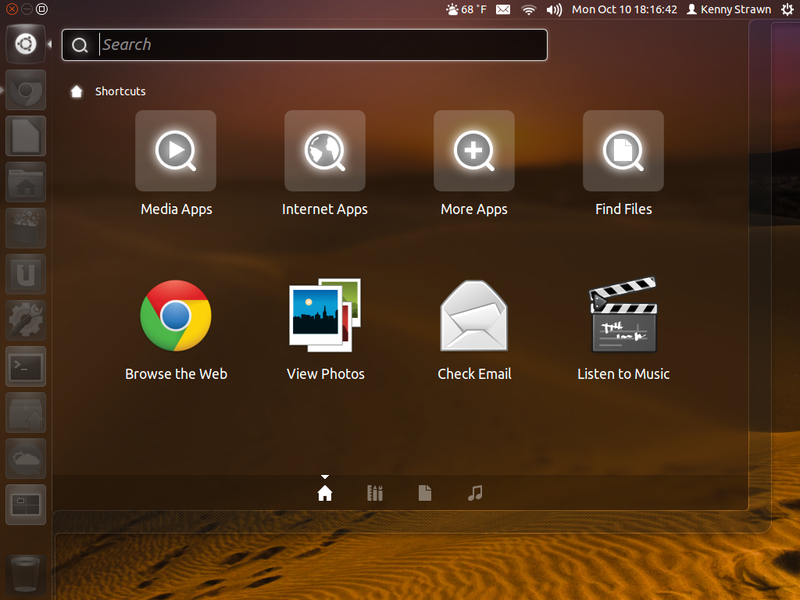
\includegraphics[width=0.8\linewidth]{images/Unity-2011}
    \caption{Unity en 2011}
  \end{figure}
\end{frame}
%% -------------

\section{Ubuntu}
\subsection*{Version}
\begin{frame}

\begin{figure}

\includegraphics[width=0.55\linewidth]{images/Ubuntu_logo}
\end{figure}

Environ 25 millions d'utilisateurs

\begin{block}{\bf Ubuntu 10.04 LTS :}

Nom de code : \textit{Lucid Lynx}

LTS : Long terme support (mars 2013)

D\'emarrage en $10s$ avec un netbook poss\'edant un DD en SSD.

\end{block}

\begin{exampleblock}{Derni\`ere version :}
Ubuntu 11.10, \textit{Oneiric Ocelot}, Unity remplace Gnome
\end{exampleblock}

\begin{alertblock}{Prochaine version :}
 Ubuntu 12.04 LTS, \textit{Precise Pangolin}
\end{alertblock}

\end{frame}

\subsection*{11.10}
\begin{frame}

  \begin{center}
    {\bf Ubuntu 11.04 / 11.10\\
    Natty Narwhal / Oneiric Ocelot}
  \end{center}

  \begin{center}
    PC \& Tablette
  \end{center}

  \begin{figure}
    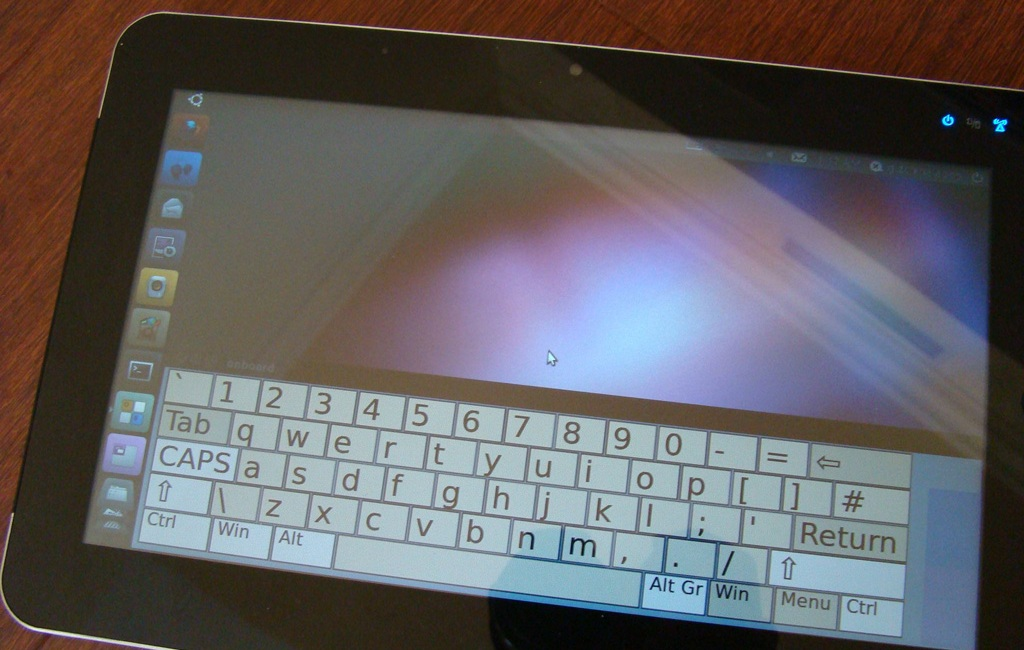
\includegraphics[width=0.7\linewidth]{images/tablette}
    \caption{Natty Narwhal sur une tablette tactile}
  \end{figure}
\end{frame}

\subsection*{Plateformes}
\begin{frame}
\begin{tabular}{c c}
\begin{minipage}{0.55\linewidth}
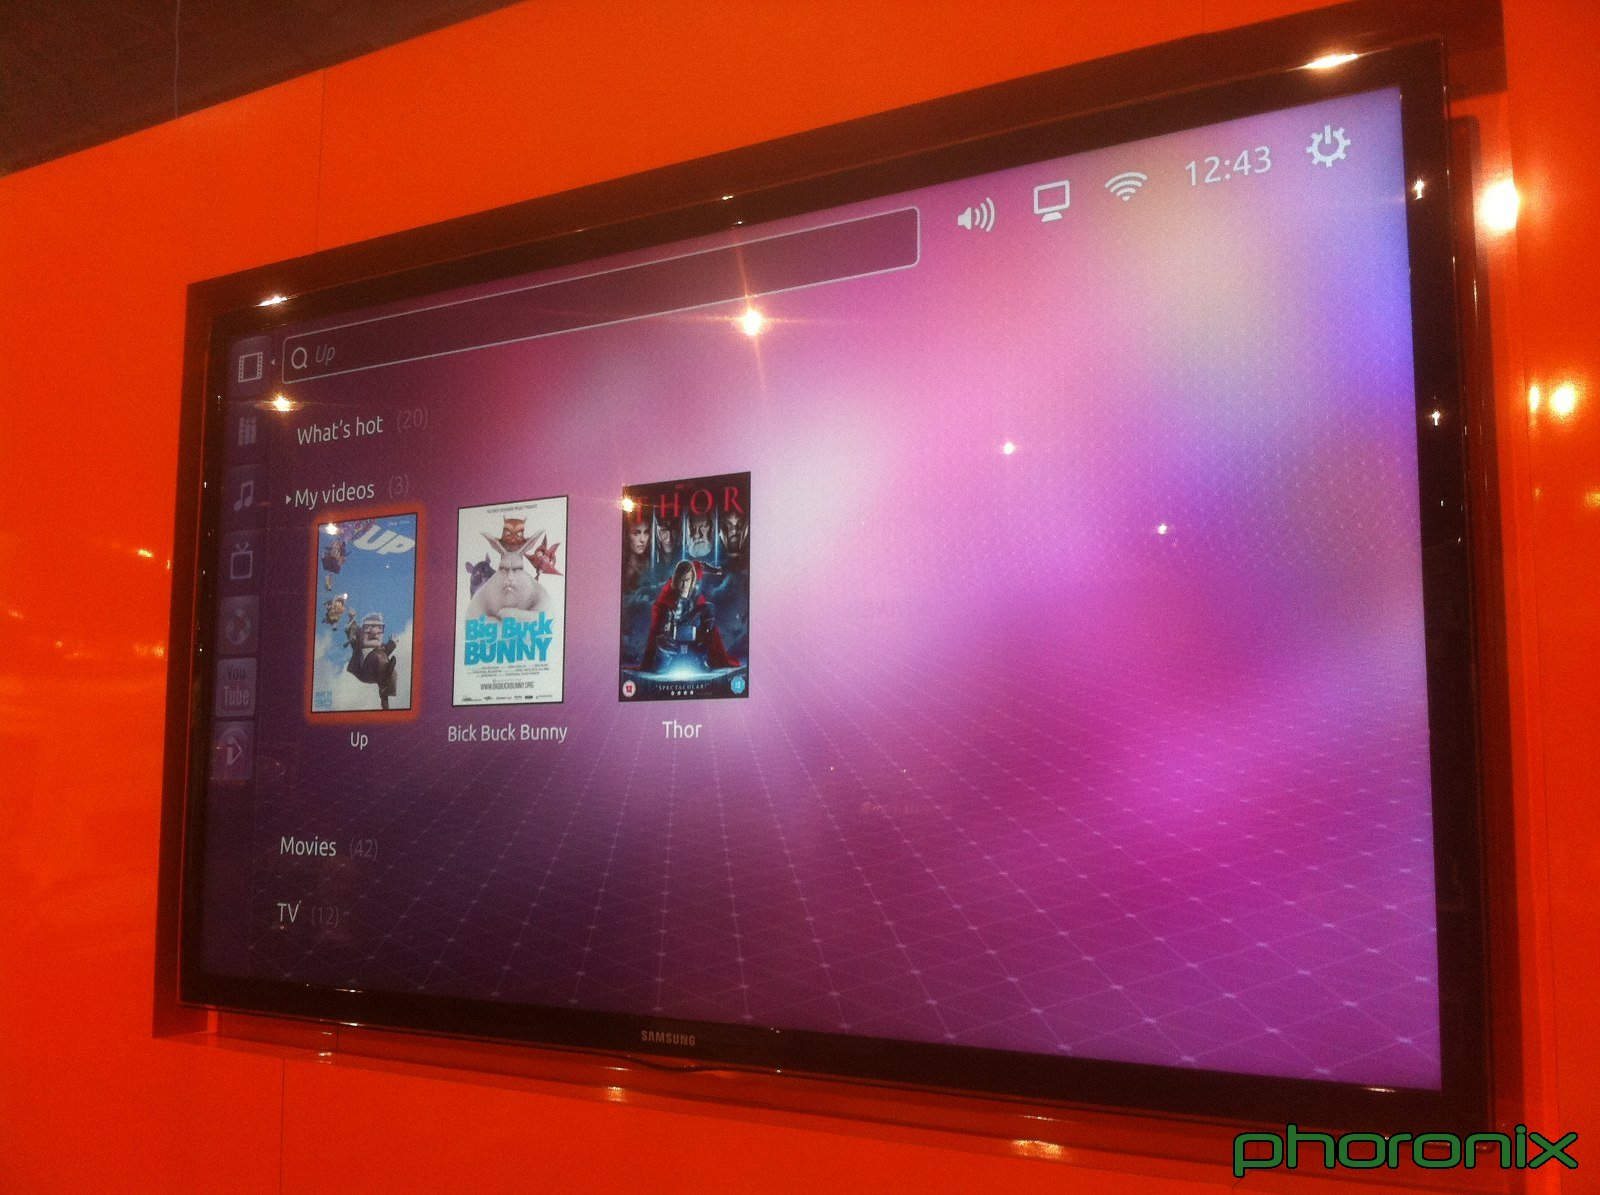
\includegraphics[width=\linewidth]{images/tv}
\end{minipage}
&
\begin{minipage}{0.4\linewidth}
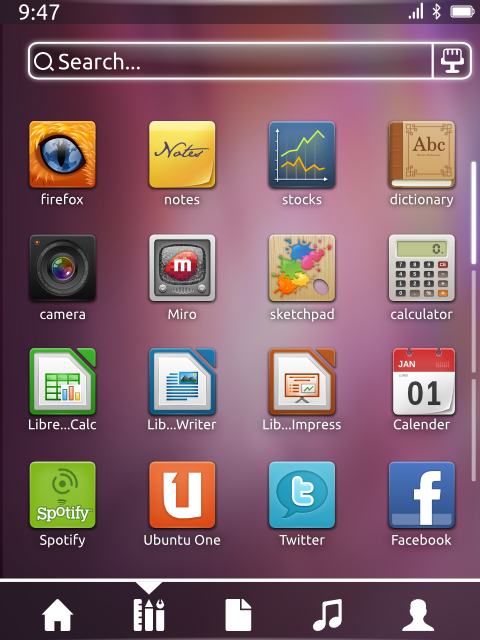
\includegraphics[width=\linewidth]{images/phone}
\end{minipage}
\end{tabular}
\end{frame}

\section{Utilisation quotidienne}

\subsection{Installer un logiciel}
\begin{frame}
  \begin{tabular}{c c}
    \begin{minipage}{0.4\linewidth}
      \begin{block}{Console}
        \small apt-cache search [name]\\
        sudo apt-get install [name]
      \end{block}
      \vspace{-2mm}
      \begin{block}{Package}
        \small Gestionnaire de paquet Synaptic
      \end{block}
      \vspace{-2mm}
      \begin{block}{Interface graphique}
        \small Logith\`eque
      \end{block}
      \vspace{2mm}
      %\hline
      %\vspace{-2mm}
      \begin{block}{Paquet debian}
       \small Installateur
      \end{block}
      \vspace{-2mm}
      \begin{block}{Manuellement}
        \small Compilation des fichiers sources
      \end{block}
    \end{minipage}
    &
    \begin{minipage}{0.6\linewidth}
      \begin{center}
      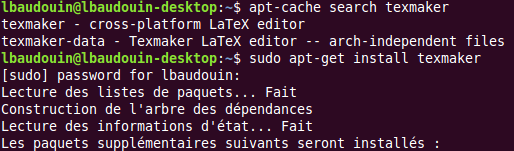
\includegraphics[width=\linewidth]{images/apt-get}\\
      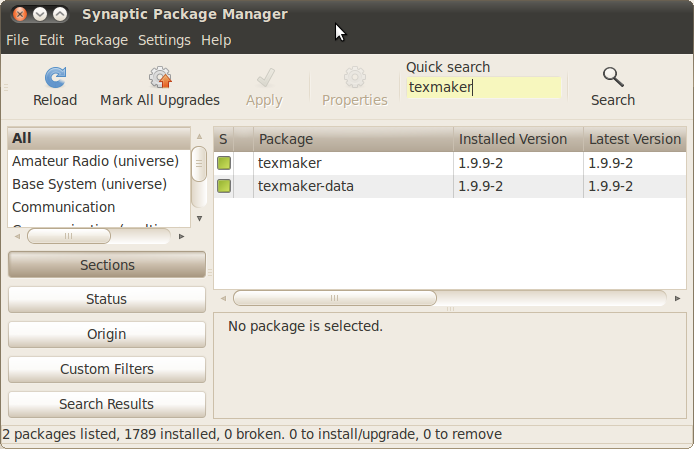
\includegraphics[width=0.9\linewidth]{images/Synaptic}\\
      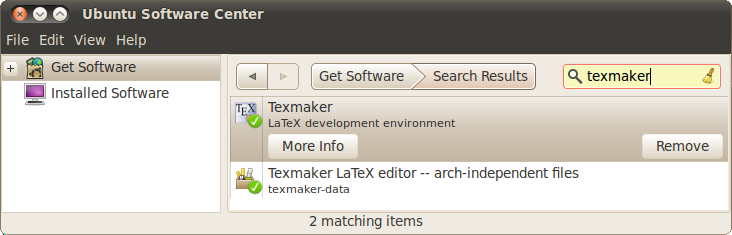
\includegraphics[width=\linewidth]{images/Logitheque}
      \end{center}
    \end{minipage}
  \end{tabular}
\end{frame}

\subsection*{D\'ependances}
\begin{frame}
	\begin{center}
		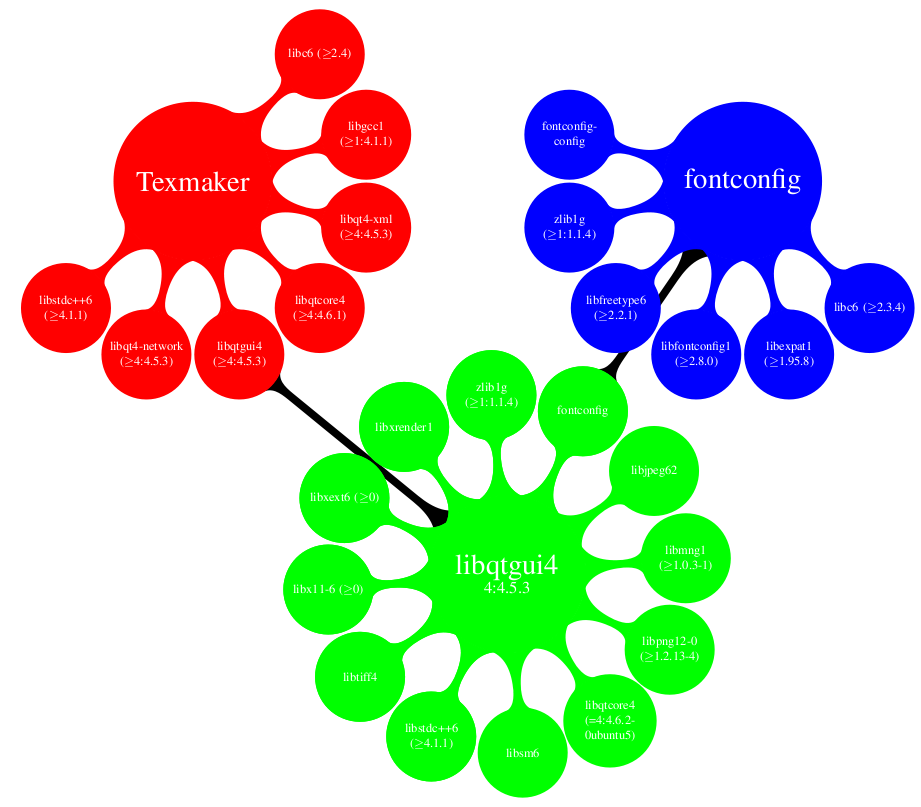
\includegraphics[width=0.9\linewidth]{images/depends}
	\end{center}
\end{frame}

\subsection{Mise \`a jour}
\begin{frame}

\begin{tabular}{l c}
	\begin{minipage}{0.4\linewidth}
	\begin{block}{Avantage}
	Mises à jour centralisées\\
	Signatures numériques
	\end{block}
  \begin{block}{Console}
    \small sudo apt-get update\\
    sudo apt-get upgrade
  \end{block}
  \begin{block}{Interface Graphique}
  Via le menu principal
  \end{block}
  \end{minipage} &
  \begin{minipage}{0.6\linewidth}
  \center 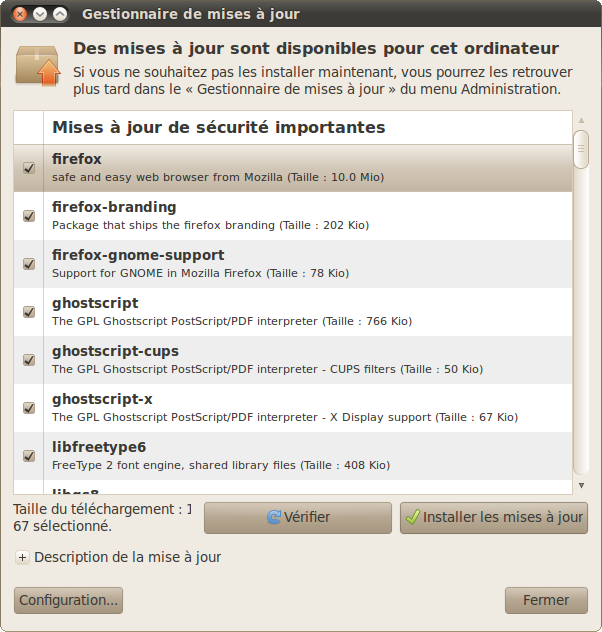
\includegraphics[width=\linewidth]{images/maj}
  \end{minipage}
  \end{tabular}
\end{frame}

\subsection{Bureautique}
\begin{frame}
  \begin{tabular}{c c}
    \begin{minipage}{0.4\linewidth}
      \begin{block}{Office}
        Open Office\\
        Libre Office...
      \end{block}
      \begin{block}{Image}
        The GIMP\\
        F-Spot...
      \end{block}
      \begin{block}{Vid\'eo}
        HandBrake\\
        Kdenlive...
      \end{block}
      \begin{block}{Internet}
        Firefox\\
        Google Chrome...
      \end{block}
    \end{minipage}
    &
    \begin{minipage}{0.5\linewidth}
    \begin{center}
    
\includegraphics[width=0.8\linewidth]{images/tux}
    \end{center}
    \end{minipage}
  \end{tabular}
\end{frame}


\subsection{Utilisateurs}
\begin{frame}

\begin{tabular}{c c}
\begin{minipage}{0.5\linewidth}
\begin{itemize}
\item Utilisateurs classiques
\item Super-utilisateur
\end{itemize}
\end{minipage}
&
\begin{minipage}{0.5\linewidth}
\begin{itemize}
\item Groupes
\item Multi-utilisateur
\end{itemize}
\end{minipage}
\end{tabular}

\begin{center}
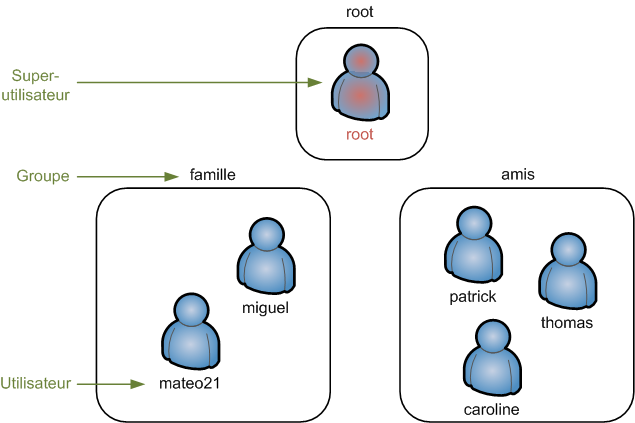
\includegraphics[width=0.8\linewidth]{images/su}
\end{center}

\end{frame}


\subsection{Utilisation avancée}
\begin{frame}
\begin{block}{Fonctions basiques}
\begin{itemize}
\item sed -i 's/oui/non/g' fichier.txt
\item mencoder Vidéo.avi -o Petite.avi -oac copy -ovc x264
\item pdftk file1.pdf file2.pdf cat output file.pdf
\item for i in *.wav ;do echo \${i\%.wav} \&\& lame -h "\${i\%.wav}.wav" "\${i\%.wav}.mp3"; done
\item find . -name *.jpg
\end{itemize}
\end{block}
\begin{block}{Aide}
\begin{itemize}
\item man sed
\item sed -h
\end{itemize}
\end{block}
\end{frame}

\subsection*{Laboratoire}
\begin{frame}
\hspace{-8mm}\begin{minipage}{\linewidth}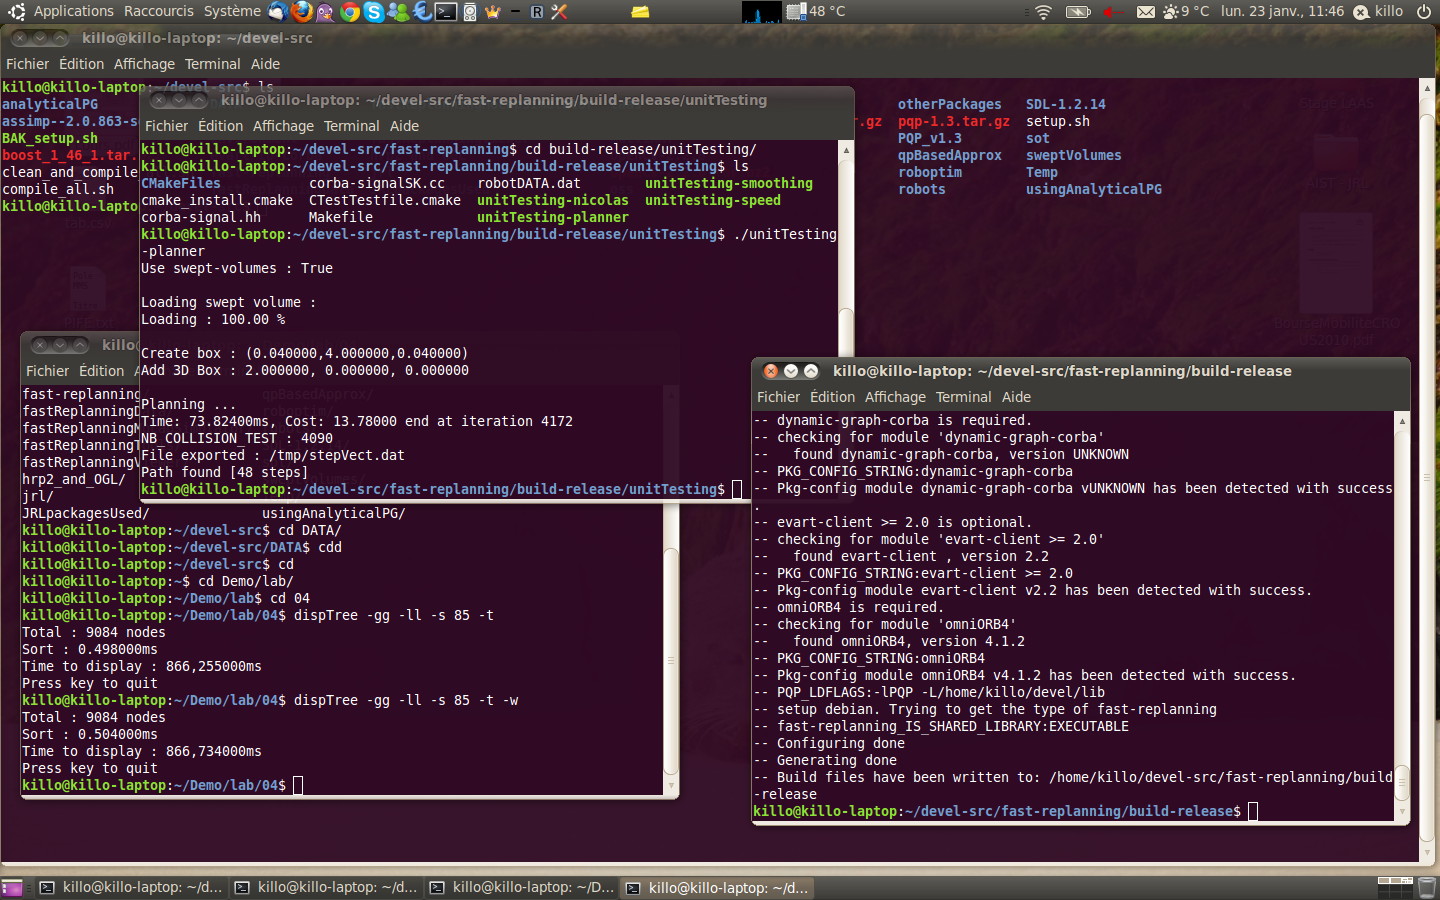
\includegraphics[width=1.15\linewidth]{images/Boulot}\end{minipage}
\end{frame}
%% -------------

\section{Comparaison avec Windows}
\subsection{Avantages de Windows}
\begin{frame} 
  \begin{flushright}
      
\includegraphics[width=0.3\linewidth]{images/Windows_logo}
  \end{flushright}
  \begin{itemize}
  \item 95\% du parc informatique personnel mondial
  \item Pr\'e-installation\footnote{ \begin{scriptsize}Vente liée, interdite en France par l'article L122-11 du Code de la consommation\end{scriptsize}}
  \item Logiciels uniquement sous Windows
  \item Jeux vid\'eo
  \item Auto-configuration multi-\'ecrans
  \item Support mat\'eriel
  \end{itemize}
\end{frame}

\subsection{Avantages de Linux}
\begin{frame} 
  \begin{flushright}
      
\includegraphics[width=0.3\linewidth]{images/Ubuntu_logo}
  \end{flushright}
  \begin{itemize}
  \item Prix imbattable
  \item Mises \`a jour centralis\'ees sans red\'emarrage
  \item Ressources / Performances
  \item S\'ecurit\'e
  \item Personnalisation / Langue
  \item Virus, spywares, trojans\footnote{{\scriptsize 800/an, contre plus de 150.000 pour Windows}}
  \item Multi-utilisateurs
  %\item Outils de d\'eveloppement int\'egr\'es
  \end{itemize}
\end{frame}

\subsection{Ressemblances}
\begin{frame}
  
  \begin{center}
\begin{tabular}{c | c}
    
\includegraphics[width=0.3\linewidth]{images/Windows_logo}&
\includegraphics[width=0.25\linewidth]{images/Ubuntu_logo}
\end{tabular}
  \end{center}

  \begin{itemize}
  \item Bureau
  \item Pack Office
  \item Navigation dans les fichiers
  \item Navigation Internet (Firefox / Chrome)
  \item Lecteur Vid\'eo / Musique
  \item MSN / Skype /
  \item ...\footnote{Avec Wine, voir \url{http://appdb.winehq.org/}}
  \end{itemize}
\end{frame}

%% -------------

\section{Conclusion}
\begin{frame}
  \begin{center}
    {\bf \huge Conclusion}
  \end{center}
  %\vspace{3mm}

  \begin{center}
    Linux peut remplacer Windows pour un usage courant mais pas encore totalement pour un usage professionnel n\'ecessitant l'utilisation de logiciels propri\'etaires précis.
\end{center}

  \begin{block}{ Solution pour un Ifmalien :}
    \textit{Dual-boot} :
    \begin{itemize}
    \item Windows 7 : Catia + certains jeux-vid\'eo
    \item Ubuntu 10.04 LTS : Pour le reste
    \end{itemize}
  \end{block}
\end{frame}

\subsection*{Sites web importants}
\begin{frame}

	{\centering {\bf {\Huge Important}}}
	\begin{block}{T\'el\'echargement}
	\url{http://ubuntu-fr.org/}\\
	\url{http://www.ubuntu.com/}
	\end{block}
	\begin{block}{Entre-aide}
	\url{http://doc.ubuntu-fr.org/}\\
	\url{http://forum.ubuntu-fr.org/}\\
	\url{http://parrains.linux.free.fr/index.php}\\
	IRC : {\tt \#{}ubuntu-fr}
	\end{block}
\end{frame}

\section{Atelier}
\begin{frame}
  {Installation}

  \begin{block}{Depuis un CD ou une clef USB :}
    \begin{itemize}
    \item Essayer Ubuntu
    \item Installer Ubuntu
    \end{itemize}
  \end{block}
  
  \begin{block}{Depuis Windows}
	  \begin{itemize}
	  \item Installation de Wubi
	 % \item Installation d'Ubuntu
	  \end{itemize}
  \end{block}

  \begin{block}{Depuis VirtualBox et un ISO:}
    \begin{itemize}
    \item Installation d'une machine vituelle
    \item Installation d'Ubuntu
    \end{itemize}
  \end{block}
 
  \begin{block}{Cr\'eation d'une partition pour Linux}
    \begin{itemize}
    \item Partitionner le disque dur
    \item Installer Windows avant Linux
    \end{itemize}
  \end{block}

\end{frame}

\end{document}  
